% Options for packages loaded elsewhere
\PassOptionsToPackage{unicode}{hyperref}
\PassOptionsToPackage{hyphens}{url}
%
\documentclass[
  12pt,
]{article}
\usepackage{lmodern}
\usepackage{amssymb,amsmath}
\usepackage{graphicx}
\usepackage{ifxetex,ifluatex}
\ifnum 0\ifxetex 1\fi\ifluatex 1\fi=0 % if pdftex
  \usepackage[T1]{fontenc}
  \usepackage[utf8]{inputenc}
  \usepackage{textcomp} % provide euro and other symbols
\else % if luatex or xetex
  \usepackage{unicode-math}
  \defaultfontfeatures{Scale=MatchLowercase}
  \defaultfontfeatures[\rmfamily]{Ligatures=TeX,Scale=1}
  \setmainfont[]{Hoefler Text}
  \setsansfont[]{Gill Sans}
\fi
% Use upquote if available, for straight quotes in verbatim environments
\IfFileExists{upquote.sty}{\usepackage{upquote}}{}
\IfFileExists{microtype.sty}{% use microtype if available
  \usepackage[]{microtype}
  \UseMicrotypeSet[protrusion]{basicmath} % disable protrusion for tt fonts
}{}
\makeatletter
\@ifundefined{KOMAClassName}{% if non-KOMA class
  \IfFileExists{parskip.sty}{%
    \usepackage{parskip}
  }{% else
    \setlength{\parindent}{0pt}
    \setlength{\parskip}{6pt plus 2pt minus 1pt}}
}{% if KOMA class
  \KOMAoptions{parskip=half}}
\makeatother
\usepackage{xcolor}
\IfFileExists{xurl.sty}{\usepackage{xurl}}{} % add URL line breaks if available
\IfFileExists{bookmark.sty}{\usepackage{bookmark}}{\usepackage{hyperref}}
\hypersetup{
  pdftitle={English Department Undergraduate Courses},
  hidelinks,
  pdfcreator={LaTeX via pandoc}}
\urlstyle{same} % disable monospaced font for URLs
\usepackage[paperheight=8.5in,paperwidth=5.5in,bottom=0.75in,top=0.75in,left=0.5in,right=0.5in]{geometry}
\setlength{\emergencystretch}{3em} % prevent overfull lines
\providecommand{\tightlist}{%
  \setlength{\itemsep}{0pt}\setlength{\parskip}{0pt}}
\setcounter{secnumdepth}{-\maxdimen} % remove section numbering
\ifluatex
  \usepackage{selnolig}  % disable illegal ligatures
\fi


\newlength{\cslhangindent}
\setlength{\cslhangindent}{1.5em}
\newlength{\csllabelwidth}
\setlength{\csllabelwidth}{3em}
\newlength{\cslentryspacingunit} % times entry-spacing
\setlength{\cslentryspacingunit}{\parskip}
\newenvironment{CSLReferences}[2] % #1 hanging-ident, #2 entry spacing
 {% don't indent paragraphs
  \setlength{\parindent}{0pt}
  % turn on hanging indent if param 1 is 1
  \ifodd #1
  \let\oldpar\par
  \def\par{\hangindent=\cslhangindent\oldpar}
  \fi
  % set entry spacing
  \setlength{\parskip}{#2\cslentryspacingunit}
 }%
 {}
\usepackage{calc}
\newcommand{\CSLBlock}[1]{#1\hfill\break}
\newcommand{\CSLLeftMargin}[1]{\parbox[t]{\csllabelwidth}{#1}}
\newcommand{\CSLRightInline}[1]{\parbox[t]{\linewidth - \csllabelwidth}{#1}\break}
\newcommand{\CSLIndent}[1]{\hspace{\cslhangindent}#1}

\usepackage{multicol}


\title{Typography versus Hitler---The Book Production War Economy
Agreement}
\author{}
\date{}

\begin{document}

\par\begin{figure}\centering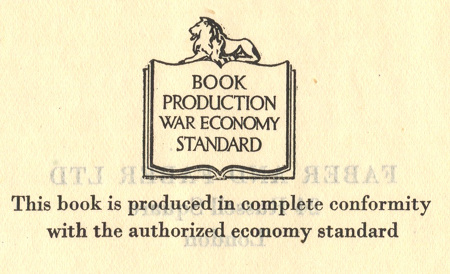
\includegraphics[width=\columnwidth]{_images/bpwes-logo.jpg}\caption{Book Production War Economy Standard Logo}\end{figure}

This post is a summary of some things I learned trying to understand
what the logo above means, after I discovered it on the copyright page
of \emph{Introducing James Joyce} (1942). \emph{Introducing} is a brief
selection of Joyce's works (including selections from \emph{Dubliners},
\emph{Portrait}, \emph{Ulysses}, and \emph{Finnegans Wake}) selected and
introduced (very briefly) by T. S. Eliot.

\par\begin{figure}\centering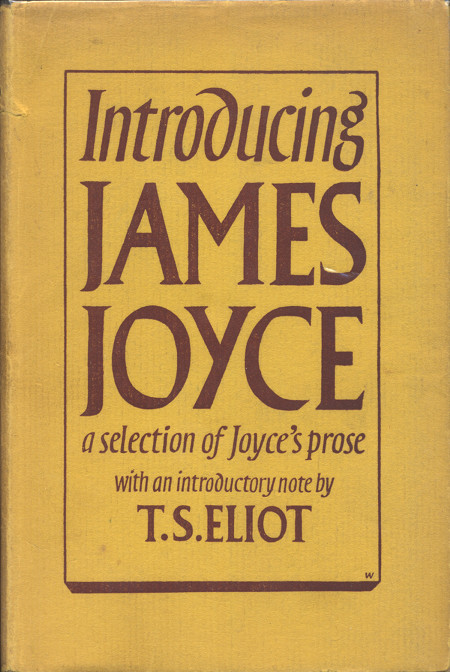
\includegraphics[width=\columnwidth]{_images/introducing_cover.jpg}\caption{“Introducing James Joyce” Dust Jacket”}\end{figure}

\hypertarget{the-book-production-war-econcomy-standard}{%
\subsection{The Book Production War Econcomy
Standard}\label{the-book-production-war-econcomy-standard}}

The British War Economy Standard was established as a way of saving
paper during the Second World War and economizing book production.
Indeed, even as the war drove up \emph{demand} for
books\protect\hyperlink{tvh-footnote1}{1}, the supply of books was
constricted drastically. This reduced supply of books owes to a number
of factors (a reduced labor force as individuals enlisted; a shift in
printing capacity to military projects, etc.), but chief among them was
the rationing of paper.\protect\hyperlink{tvh-footnote2}{2} In England,

\begin{quote}
Paper was rationed, beginning in March 1940, when publishers were
allowed only 60 percent of what they had used in 1938-39. The proportion
fell to 37.5 percent by January 1, 1942, when the Book Production War
Economy Agreement took effect. The scheme mandated smaller type, less
white space, and inferior papers and bindings. It resulted in some
remarkably ugly books, but it conserved raw materials. (Rose 351)
\end{quote}

While rationing occurred in the United States, under the direction of
the War Production Board, rules for paper use seem to have been
comparatively liberal.\protect\hyperlink{tvh-footnote3}{3} In Britain,
by contrast, a more severe shortage led to the Book Production War
Economy Agreement---an agreement between the British government and
publishers which apportioned paper among publishers (based on their
1938-39 usage\protect\hyperlink{tvh-footnote4}{4}) and spelled out
standards for paper conservation. {Valerie Holman's \emph{Print for
Victory} tells the story of books in England during the second World War
in detail, and includes extension discussions of the BPWEA. As an
appendeix, she includes some of the details of the BPWEA. It is my chief
source in this post; its a great work with truly excellent
illustrations.}

The BPWEA included a variety of measures for reducing, and
rationalizing, paper use. For instance, as the war continued, a process
evolved for prioritizing certain types of books over others (by
affording an additional paper ration for books deemed ``essential,'' see
Holman 83\emph{ff}). But it also included rules for making the most
efficient use of each page: ``Publishers decided to focus their
attention on the printed page, looking at books not as they were, but as
they might be if less white space surrounded the text and the type size
was reduced so that more could be printed on less paper'' (Holman 72).

\hypertarget{measuring-paper-use}{%
\subsection{Measuring Paper Use}\label{measuring-paper-use}}

The BPWEA established rules for the maximum weight of paper and boards
for binding.{The weights both are based on the weight of a ream of quad
crown---40''x30''---sheets. Which is not an easy measure to imagine,
unless you happen to have a paper factory handy.} It also required:

\begin{itemize}
\tightlist
\item
  ``preliminary matter'' must not exceed four pages (introductions,
  tables of contents, and so on may be regarded as part of the text, not
  preliminary matter)
\item
  Chapter Headings and Breaks ``must not be extravagantly displayed and
  must start not lower on the page than the height of the third line of
  the text on a full page. There must be no blank page between chapters.
  In fiction, chapters must be run on with a gap of not more than eight
  lines\ldots{}'' (qtd. in Holman 271).
\end{itemize}

For instance, this volume, \emph{USSR: Her Life and People}, published
in 1943 under the BPWAE, shows a chapter break that is decidedly not
extravagant:

\par\begin{figure}\centering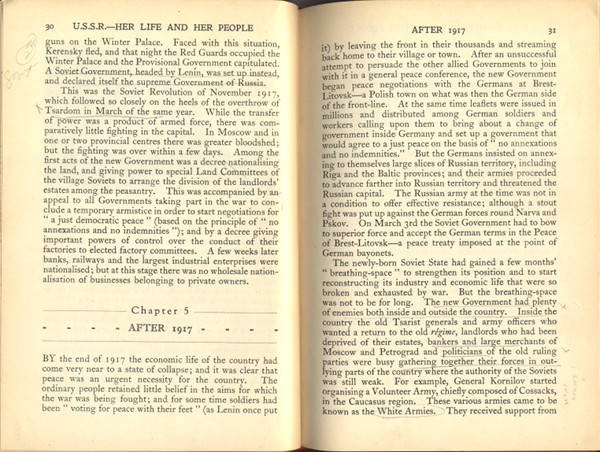
\includegraphics[width=\columnwidth]{_images/ussr_pages30-31.jpg}\caption{An Opening from “USSR: Her Life and People,” showing a Chapter Heading}\end{figure}

Additionally a book must meet one of two ``typographical standards'':

\begin{enumerate}
\def\labelenumi{\arabic{enumi}.}
\item
  \emph{Type-to-page Ratio and Maximum Type Size}: ``The percentage of
  type-area to the page-area (untrimmed) must not be less than 58 per
  cent'' (Holman 268). Additionally, this provision specifices maximum
  type sizes and leading; thus a book measuring 8.75'' by 5.625''---a
  demy octavo---or larger can have type no larger than 11 point, with 1
  point leading. A small book (smaller than crown ocatvo, 7.5'' by
  5in'') must have type set no small than 11 pt, with (!) no leading.
  (The agreement includes exceptions for Children's and Educational
  Books, as well as for books under 64 pages).
\item
  \emph{Minimum Words per Page}: Alternatively, one could meet the
  typographic standards by demonstrating a minimum number of words per
  page. The type-area must be a minimum of 55 (rather than 58) percent
  of the page; but one must also meet a minimum number of words per page
  based on format (e.g.~478 words per page for a page measuring 8.75''
  by 5.625''; 375 for a crown octavo volume, etc). It also includes a
  procedure for estimating words per page.
\end{enumerate}

A book had to meet \emph{one} of those two typographical
standards---meaning, in effect, a publisher could choose to have wider
margins but guarantee a certain number of words per page (the second
standard), or a publisher could decide to have smaller margins (a larger
type-area and type-to-page ratio) and stick with specified contraints
for type size and leading.

Additionally, there were other exceptions: for works printed for export;
for books printed as part of a pre-existing multivolume set or series,
etc.

Did these contraints produce, as Rose suggests, ``some remarkably ugly
books''? The effects of these requirements were significant enough that
one member of the Publisher's War Emergency Committee worried that the
standard was making books unreadable: ``We must at all costs study the
eyesight of readers,'' he wrote in a letter to the Board of Trade at the
beginning of 1943, ``Already I have received complaints from our own
Services and from the American Services that the type used in many of
our books is too small'' (qtd. in Holman 74).

What does this look like in practice? Here is a page from
\emph{Introducing James Joyce}:

\par\begin{figure}\centering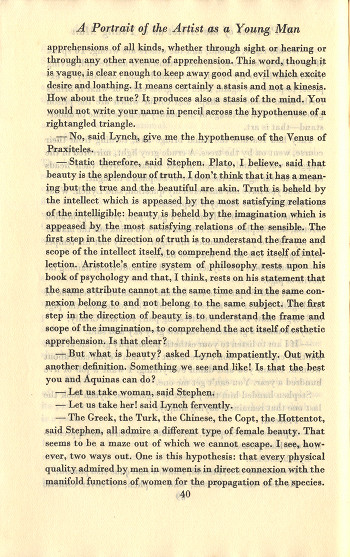
\includegraphics[width=\columnwidth]{_images/introducing_page40.jpg}\caption{Page 40 of “Introducing James Joyce”}\end{figure}

One can feel the difference in the book: it is very thin; the boards are
light (it has an unusual degree of bend for a book published in boards,
feeling halfway between a hardcover and paperback). It has very little
preliminary matter: the book has a blank free endpaper, a half-title
page (with blank verso), and a title page (with copyright information
and BPWEA statement on the verso) before the main text begins. The paper
is indeed thin; if you look closely you can see through the page, to the
type on the opposite side of the page.

\par\begin{figure}\centering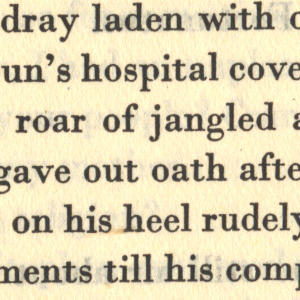
\includegraphics[width=\columnwidth]{_images/introducing_1inch-square.jpg}\caption{One Inch Square of “Introducing James Joyce”}\end{figure}

And what about the typographical standards? The page measures 7 inches
by 4.75 inches. According to the BPWEA, it must have a minimum of 332.5
words per page. {That calculation is made by multiplying the total area
of the page by 10 words per square inch; the BPWEA specifices a slightly
different requirement of words/in\^{}2 for other formats.} Per the
BPWEA, estimatation of the number of words per page for a volume must be
based on a count of 10 consecutive lines, taken from 10 random pages.
For \emph{Introducing Joyce} I got an average of 106.5 words per ten
lines; 35 lines per page, means an average of 372.75 words per page.
This figure is well above the BPWEA requirement; I imagine that the
excerpts from \emph{Finnegans Wake} contribute to surprisingly large
number (they have very few paragraph breaks or short lines, and so have
consistently full lines).

\emph{Introducing Joyce} also meets the type-to-page ratio. By my
measurement, the type area is 62.5\% of the page area.

For comparison, consider this page from \emph{Boot and Saddle in
Africa}, published in 1943 (when the BPWEA was in full swing), but
published and printed in the US.

\par\begin{figure}\centering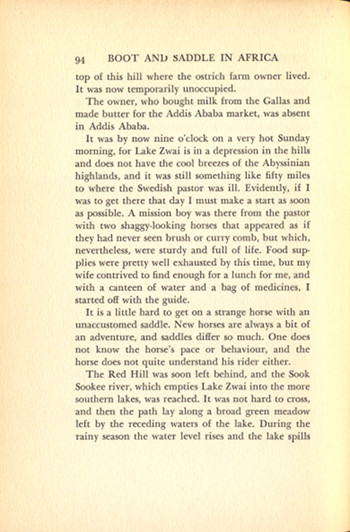
\includegraphics[width=\columnwidth]{_images/boot-and-saddle_pg94.jpg}\caption{A Page of “Boot and Saddle in Africa”}\end{figure}

It's copyright page declares that ``This book has been manufactured in
this form in compliance with orders of the War Production Board for the
conservation of paper and other materials necessary for the prosecution
of the War.'' Yet, these requirements were far less stringent than their
British counterparts. The paper of this volume is heavier (obvious in
the image below), and the leading is visibly greater; chapters are
started on a new page. By my measurement the type-space takes up only
47\% of the page, and so fails the type-to-page requirement. The pages
measure 5.5'' by 8'', placing it in the same category of format as
\emph{Introducing James Joyce}---if published under the BPWEA, it should
have 10 words per square inch, or 440 words per page. Using the
estimatation formula descried in the BPWEA, however, \emph{Boot and
Saddle} has an average of 277.2 words per page.

Here are the pages side by side, with scale preserved.

\par\begin{figure}\centering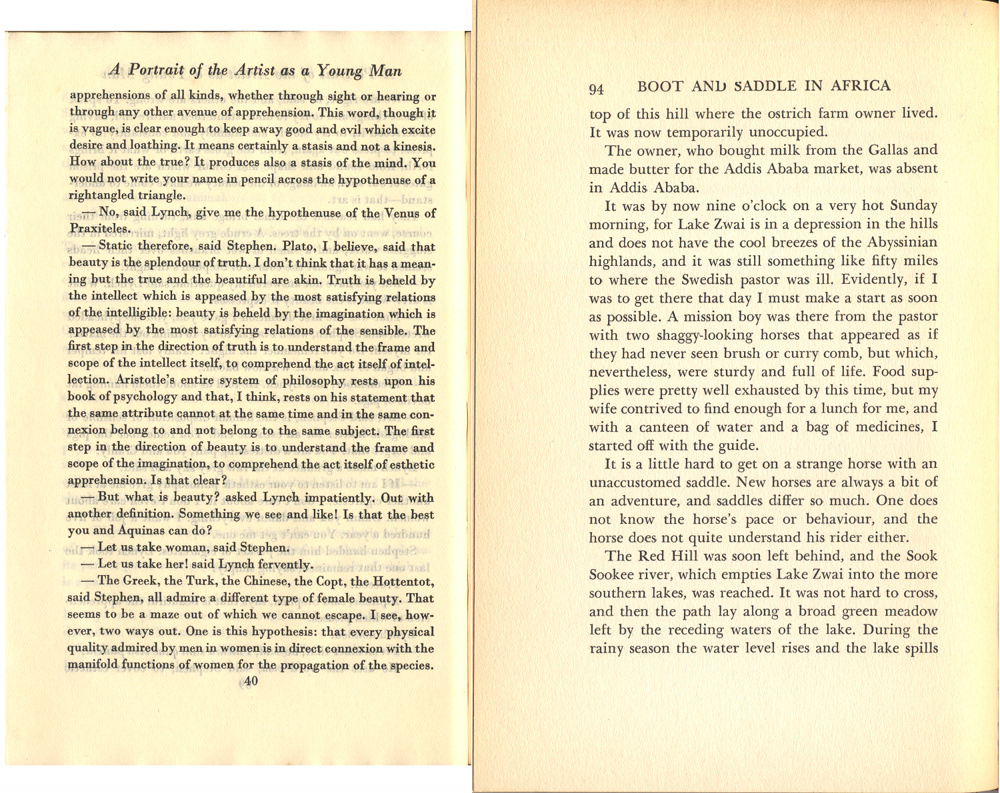
\includegraphics[width=\columnwidth]{_images/comparison.jpg}\caption{Pages of “Introducing James Joyce” and “Boot and Saddle in Africa”}\end{figure}

The type-area of \emph{Introducing} is the same size as \emph{Boot and
Saddle}, even though the page itself is much smaller. The type is
likewise much smaller.

\hypertarget{computing-paper-use}{%
\subsection{Computing Paper Use}\label{computing-paper-use}}

I was curious whether one could compare the relative amounts of ink per
page; a little bit of Python can approximate this. We have images of
pages; if we sort the pixels in each vertical column by color, we can
compare the total amount of black on one page to another. {You could
also simply sort the pixels by treating the images as a one dimensional
arrays---that is, as just lists of numbers---I found this less helpful
because the margins makes it harder to compare the images as a glance.}

Here is what the relevant bit of code looks like:

\{\% highlight python \%\} \# We use the Python Image Library from PIL
import Image

\hypertarget{open-the-image-in-png-format.}{%
\section{Open the image, in PNG
format.}\label{open-the-image-in-png-format.}}

image = Image.open(`introducing-james-joyce\_page90.png')

\hypertarget{load-the-pixel-data-from-the-image-into}{%
\section{Load the pixel data from the image
into}\label{load-the-pixel-data-from-the-image-into}}

\hypertarget{a-list-we-can-manipulate.}{%
\section{a list we can manipulate.}\label{a-list-we-can-manipulate.}}

pixels = list(image.getdata())

\hypertarget{get-the-dimensions-of-the-image-image-provides-a-tuple}{%
\section{Get the dimensions of the image; Image provides a
tuple}\label{get-the-dimensions-of-the-image-image-provides-a-tuple}}

(width, height) = image.size

\hypertarget{in-order-to-sort-by-column-we-will-extract-each-column}{%
\section{In order to sort by column, we will extract each
column}\label{in-order-to-sort-by-column-we-will-extract-each-column}}

\hypertarget{of-the-image-separately-and-then-sort-it.}{%
\section{of the image separately and then sort
it.}\label{of-the-image-separately-and-then-sort-it.}}

\hypertarget{first-loop-through-each-column-in-the-images-width.}{%
\section{First, loop through each ``column'' in the image's
width.}\label{first-loop-through-each-column-in-the-images-width.}}

for column in range(0, width): \# We'll build a list for just this
column. pixelColumn = {[}{]}

\# This loop extracts the color values for a column \# by adding each
pixel, for each ``row'' within the \# current colum to a list. for pixel
in range(0, height): pixelColumn.append(pixels{[}x*width+column{]})

\# Now we sort the list we just generated. \# The ``sorting'' I leave to
a built-in Python function. pixelColumn =
sorted(pixelColumn,reverse=True)

\# Now our data is sorted, but its in a list, divorced \# from the rest
of the image. We need to load it back \# into the image itself; we use
the same loop as before \# but moving the now re-ordereddata in the
opposite \# direction. for pixel in range(0, height):
pixels{[}x*width+column{]} = pixelColumn{[}pixel{]}

\hypertarget{and-push-that-altered-data-back-to-the-image-object}{%
\section{And push that altered data back to the Image
object,}\label{and-push-that-altered-data-back-to-the-image-object}}

\hypertarget{which-we-can-now-show-or-save.}{%
\section{which we can now show() or
save().}\label{which-we-can-now-show-or-save.}}

image.putdata(pixels)

\{\% endhighlight \%\}

You can see this code, modified to take a command line argument, at
\href{https://github.com/c-forster/imageAverage}{github}. (You'll need
Python and the Python Image Library installed to run it though.)

Here are the output images for the page of \emph{Introducing James
Joyce} and \emph{Boot and Saddle}:

\par\begin{figure}\centering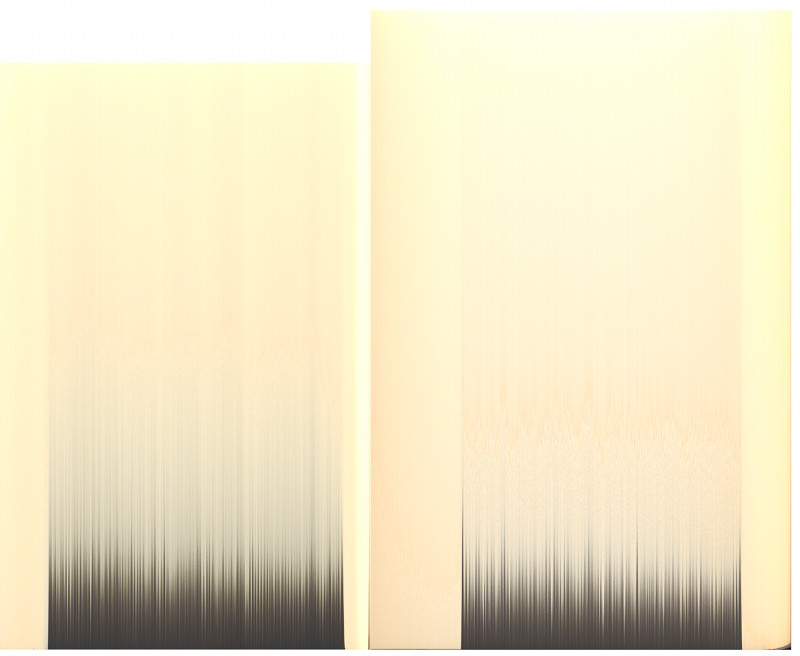
\includegraphics[width=\columnwidth]{_images/sorted-comparison.jpg}\caption{“Introducing James Joyce” and “Boot and Saddle” pages, with Columns sorted of Pixels Sorted by Color}\end{figure}

One could boil this down further to a single number using some sort of
``average'' to try to measure how much of a page is occupied by ink. For
instance, using a function described on
\href{http://stackoverflow.com/questions/3490727/what-are-some-methods-to-analyze-image-brightness-using-python}{this
StackOverflow thread}, the page of \emph{Introducing James Joyce} has a
brightness average of 219.938548387, while \emph{Boot and Saddle} is
225.179950898 {Those values, I assume, are out of 255---where 0 is
completely black and 255 is completely white.}; that greater level of
brightness represents the less crowded (or less efficiently used) page.
Though the difference in number seems rather slight and certainly
doesn't capture the difference in paper use the way the average words
per page statistic does.

This is an an odd, and not entirely successful, way of looking at this
data; the (admittedly unpleasant to perform) calculations{The numbing
image of some poor clerk or assistant counting blocks of ten lines all
day\ldots{}}) the BPWEA recommends better capture the amount of
linguistic information compressed into physical space; though the
analyses of the brightness of the images do have the advantage of
registering something that the typographical standards of the BPWEA
calculations do not: the effect of the print bleeding through the thin
paper, visible, for instance, in the middle-gray tones in the sorted
\emph{Introducing} image.

\hypertarget{book-formats-and-reading}{%
\subsection{Book Formats and Reading}\label{book-formats-and-reading}}

Of course, looking at these images, one realizes that book format and
expectations have changed quite a bit; while \emph{Introducing James
Joyce}, seems cramped on the page, and the paper is clearly \emph{too}
thin, it is still far more recognizable than \emph{Boot and Saddle}
which feels like a brick beside it---its heft and liberal use of
whitespace are actually relatively alien to a reader used to the formats
of genre novels, Bantam paperbacks, and Norton Critical Editions. The
Penguin paperback format (which, in my estimation, \emph{Introducing} is
far closer to than the older format of \emph{Boot and Saddle}) emerged
just prior to the period of these restrictions and so is certainly
\emph{not} a product of the war. One might hazard, however, that the
requirements of the BPWEA helped cement certain expectations for our
experience of the page. While, as Rose, contends, these standards
produced some ugly books, they also may have improved book design
overall. Holman notes, ``Although books published in the Second World
War are more often remembered for their typographical severity than for
their visual richness, it was a period in which the need to convey
information swiftly and succinctly placed a premium on good design''
(112).

And indeed, Brandt suggests a very specific salutary effect of the US's
own (more limited) paper rationing: {Brandt's essay is a sort of ranty
screed about how the United States is ``culturally'' ``one of the
backward nations of the world'' (88), but I'll take his observations on
book formats.}

\begin{quote}
Publishers took as a first step, and a most desirable one, the making of
\textbf{thinner books}. During the lush twenties publishers adopted the
British practice of bulking books, on the theory that bookstore
customers would feel that they were getting more for their money if the
bulk were greater. The customer naturally was confused by seeing two
books at the same price, one twice the thickness of the other; and,
unless he were truly discriminating, he tended to buy the bulkier. The
bulked book created a real space problem for libraries as well as for
the individual collectors. Under weight restrictions, publishers had to
yield to the use of lighter papers, with the result that the buyer who
was accumulating a library could afford, on a space basis, to buy more
books. (102)
\end{quote}

(I wish I knew more about the extent to which ``bulky books'' were a
``British practice,'' and what that history is.) Whether or not space
was really the premium Brandt suggests, it does seem plausible that the
restrictions of the BPWEA (and the milder American {I, of course, have
said nothing about continental book publishing, or publishing elsewhere
in the British colonies, or in Japan, or North Africa, or the Middle
East---all of which was, no doubt, affected. It is worth noting that
because of the costs under the BPWEA, some British publishers moved
their printing to India.} regime) did affect our own present
expectations for print formats.

\hypertarget{notes}{%
\subsection{Notes}\label{notes}}

\begin{itemize}
\item
  \protect\hyperlink{tvh-ref1}{1}---``The stress of World War II
  actually increased demand for books, out of a need for distraction,
  for understanding the world situation, or for somethign to do during
  long blackouts. In Halifax, public library loans jumped from 716,000
  in 1938 to just over a million in 1945\ldots{} In February 1940, 62
  percent of adults were reading a book, falling to 51 percent in 1941
  and 45 percent in 1946-7'' (Rose 350-51). I'm not entirely sure what
  that figure about adults ``reading a book'' means.
\item
  \protect\hyperlink{tvh-ref2}{2}---In part the paper shortage was a
  function of the fact that most of the paper used in British printing
  used esparto grass, imported from North Africa, then under French
  colonial control.
\item
  \protect\hyperlink{tvh-ref3}{3}---The early years of the war are
  described by Joseph Brandt as a boom-time for American book
  publishers. ``Publishers have never before enjoyed either such
  extraordinary prosperity or such extraorindary difficulties in
  producing books\ldots{} Book sales had increased in 1943 form 20 to 30
  percent over 1942, even though questions of paper rationing and
  manufacturing were assuming ever more serious proportions'' (101). The
  chief effects Brandt describes are an attempt to save paper by
  reducing paper weight. ``The War Production Board\ldots{} issued a
  curtailed order for the book-publishing industry, which in 1944 was
  increased. Publishers were permitted to use only 75 per cent of the
  weight of paper they had used in 1942'' (101-102). This is a less
  drastic reduction and one that applies only to paper weight used in
  the interest of reducing overall; it does not seem to be put an
  absolute cap on paper usage, nor does Brandt mention any specifically
  typographical requirements.
\item
  \protect\hyperlink{tvh-ref4}{4}---One rather perverse effect of this
  accounting is that a publisher who happened to have an especially good
  year in 1938-39 continued to reap the benefit of that expanded ration
  throughout the war yers and beyond. One such publisher was Hutchinson,
  who had a best-seller with Hitler's \emph{Mein Kampf} that year (see
  Holman 12, 252-254).
\end{itemize}

\hypertarget{works-cited}{%
\subsection{Works Cited}\label{works-cited}}

\begin{itemize}
\item
  Brandt, Joseph. ``War and the Book Trade.'' \emph{Book and Libraries
  in Wartime}. Ed. Pierce Butler. Chicago: U of Chicago P. 1945. Print.
\item
  Holman, Valerie. \emph{Print for Victory: Book Publishing in England,
  1939-1945}. London: British Library, 2008. Print.
\item
  Lambie, Thomas. \emph{Boot and Saddle in Africa}. Philadelphia:
  Blakiston Co.~1943. Print.
\item
  Rose, Jonathan. ``Modernity and Print I: Britain 1890-1970.'' \emph{A
  Companion to the History of the Book}. Malden, MA: Blackwell, 2007.
  341--353. Print.
\end{itemize}

\end{document}
